
\chapter{Pacific-South American pattern climatology}\label{c:psa_climatology}

%=========================================================================

\begin{synopsis}
The chapter presents a new method for objectively identifying the Pacific-South American (PSA) pattern. The method is used to characterise the climatological characteristics of the pattern and its influence on regional climate variability.
\end{synopsis}

%=====================

\section{Methodology}

The key methodological advance of the previous chapter was that in comparison to existing studies, it more fully exploited the information available from Fourier analysis. The use of the Hilbert transform to calculate the wave envelope overcame many of the limitations of existing wave identification methods, leading to a number of new insights into the climatological characteristics of the SH zonal waves and their influence on regional climate variability. Similar limitations apply to existing methods of PSA pattern identification, which means Fourier analysis may also yield new insights in that context. More specifically, identification of the PSA pattern is typically based on EOF analysis, which unlike Fourier analysis allows for only a crude representation of variations in wave phase (via the PSA-1 and PSA-2 modes, which are 90$^{\circ}$ out of phase). This has made it difficult to interpret characteristics such as the propagation of the pattern and the physical meaning of the PSA-1 and PSA-2 modes more generally. 

The use of Fourier analysis to more precisely capture the phase of the PSA pattern required further development/modification of the zonal wave methods presented in the previous chapter, which focused more on capturing spatial variations in wave amplitude. Another important difference was the fact that the path of the PSA pattern has a substantial meridional component. In some sense zonally oriented waves can be thought of as the simplest wave identification case, because Fourier analysis can be performed along lines of constant latitude. The added complexity of identifying/tracking non-zonal propagation has only just begun to be considered in the literature \citep[e.g.][]{Zimin2006,Souders2014}, with most existing climatologies of synoptic-scale Rossby waves avoiding the issue by focusing solely on zonally orientated waves \citep[e.g.][]{Glatt2014}. A key insight of the method developed here is that unlike the generalised case of all possible non-zonal propagation, analysis of the PSA pattern can make use of the fact that it follows an approximate great circle path \citep{Hoskins1981}. By rotating the global coordinate system such that the equator (itself a great circle) traces the approximate path of the PSA pattern, the identification algorithm developed here was able to simply apply Fourier analysis along the `equator' in the new zonal direction. Such grid rotation is commonly used in ocean modelling to avoid coordinate singularities caused by the convergence of meridians at the poles \citep[i.e. the grid is rotated to place the north pole over a continent; e.g.][]{Bonaventura2012}, but it had not previously been applied in the context of tropospheric wave identification.

\subsection{Identification algorithm}\label{s:psa_id}

\subsubsection{Grid rotation}

In order to align the new equator with the approximate path of the PSA pattern, a global 0.75$^{\circ}$ latitude by 0.75$^{\circ}$ longitude grid was defined (i.e. the same resolution as the original ERA-Interim data) with the north pole located at 20$^{\circ}$N, 260$^{\circ}$E. The 500 hPa zonal and meridional wind data were used to calculate the meridional wind relative to the new north, and then the temporal anomaly of this new meridional wind was linearly interpolated to the rotated grid for use in the Fourier analysis (e.g. Figure \ref{fig:rotation}). It should be noted that zonal wave studies (e.g. Chapter \ref{c:zw_climatology}) tend to skip this final step of calculating the anomaly, because in the case of zonal waves the temporal mean of the meridional wind is typically close to zero (and hence waveforms defined by the meridional wind already oscillate about zero). 

On this rotated grid, the search region of interest was defined as the area bounded by 10$^{\circ}$S to 10$^{\circ}$N and 115$^{\circ}$E to 235$^{\circ}$E (this approximate area is referred to as the PSA sector at times throughout the thesis). This region (and associated north pole location) was selected via visual comparison with existing definitions of the PSA pattern (e.g. Figure \ref{fig:eof}), however the final results were not sensitive to small changes in pole location or search region bounds.

\begin{figure}
\begin{center}
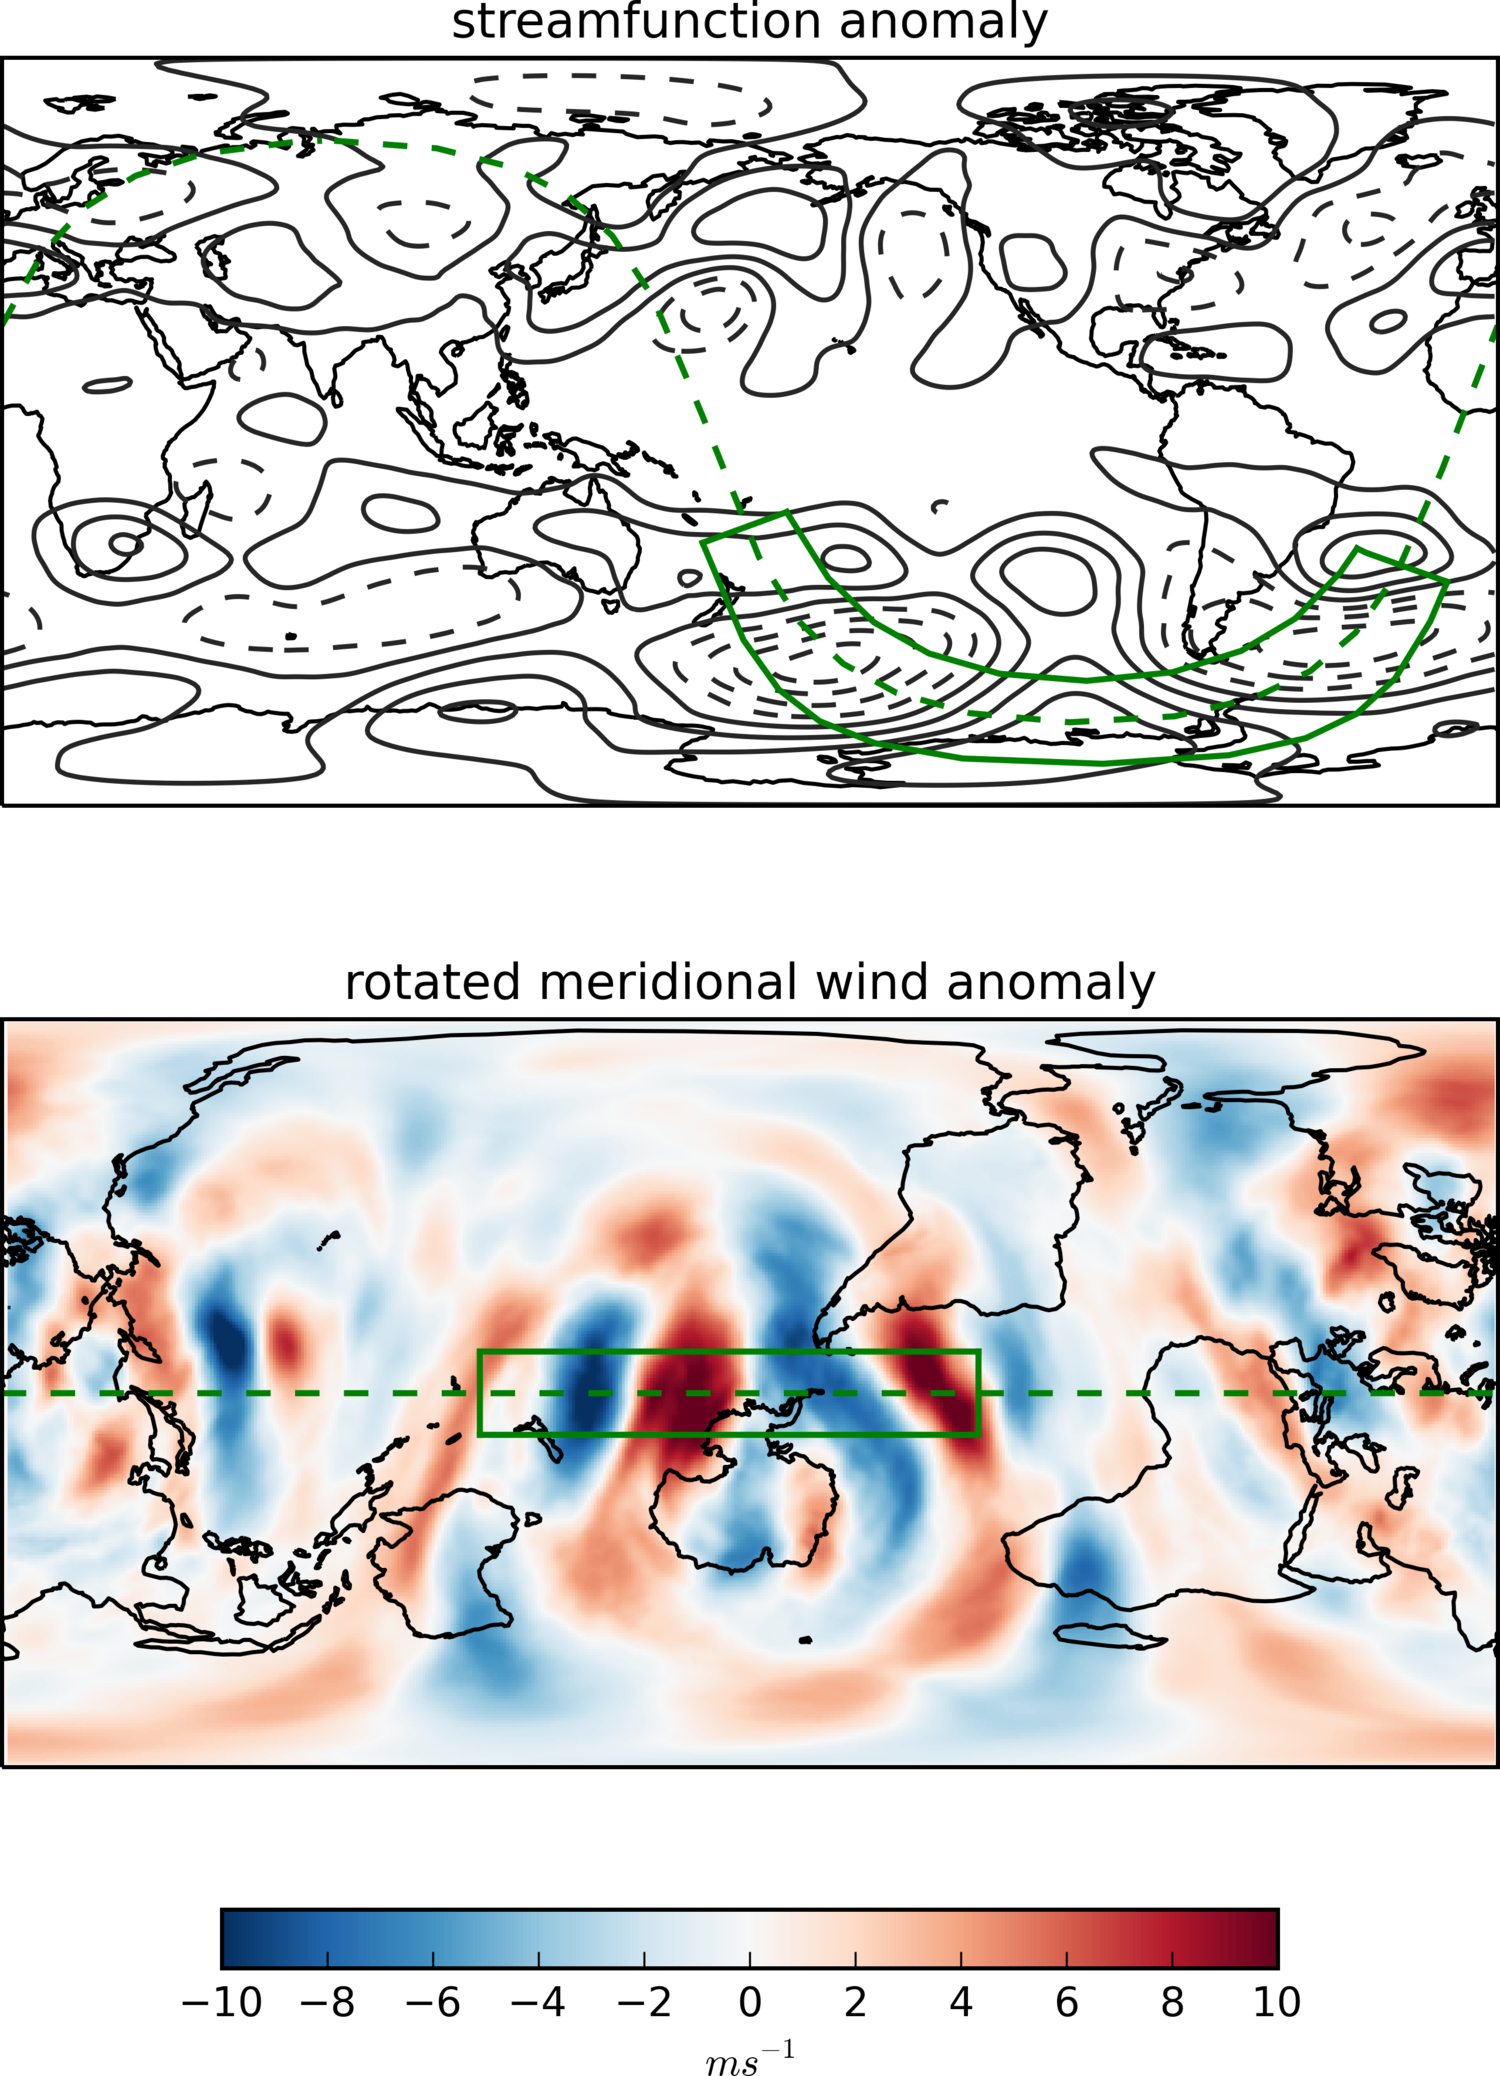
\includegraphics[width=0.7\columnwidth]{figures/psa/Figure4-1.png}
\caption[Coordinate system rotation and corresponding 500 hPa meridional wind conversion for a 30 day mean centred on 18 May 2006]{\label{fig:rotation}
Atmospheric circulation at 500 hPa for a 30 day mean centred on 18 May 2006. The top panel shows the streamfunction anomaly plotted on a regular global grid (dashed contours indicate negative values and the contour interval is $3.0 \times 10^6 \: m^2 s^{-1}$), while the bottom panel shows the corresponding meridional wind anomaly on a rotated grid where the north pole is located at 20$^{\circ}$N, 260$^{\circ}$E. The solid green box is bounded by 10$^{\circ}$S to 10$^{\circ}$N and 115$^{\circ}$E to 235$^{\circ}$E on the rotated grid and corresponds to the search region of interest (or `PSA sector'), while the green dashed line corresponds to the equator on the rotated grid.%
}
\end{center}
\end{figure}

\subsubsection{Fourier analysis}

To prepare the meridional wind anomaly for Fourier analysis, the meridional mean was calculated over 10$^{\circ}$S to 10$^{\circ}$N (in order to eliminate the latitudinal dimension) and then values outside of 115$^{\circ}$E to 235$^{\circ}$E were set to zero. Zero padding is a commonly used technique in signal processing when the waveform of interest does not complete an integer number of cycles in a given domain, and is equivalent to multiplying the original signal (in this case the meridional mean meridional wind anomaly) by a square window function. This multiplication (or convolution) of two waves has consequences in frequency space, such that even a perfectly sinusoidal signal that would repeat exactly six times (for example) over the zero padded domain would show power at more than one frequency. This phenomenon is known as spectral leakage (into the side lobes of the frequency spectrum) and arises due to the fact that a square window function is not square in frequency space. In analyses where excessive leakage is undesirable, a Hanning or Hamming window can be used instead. In the frequency space these windows do not display as much spread into the side lobes, however this comes at the expense of the magnitude of the main lobes. Since the selection process used here (see below) focuses identifying the main lobes, a square window function was considered most appropriate.

\subsubsection{Identification and characterisation of PSA-like variability}

Given that the PSA pattern completes approximately 1.6 to 2.0 cycles (depending on the specific EOF mode) over the 120$^{\circ}$ search area (see Figure \ref{fig:eof}), data times where a Fourier transform revealed wavenumber five and six as dominant frequencies over the zero padded 360$^{\circ}$ domain was the focus of this analysis. In particular, a data time was said to display PSA-like variability (and hence was selected for further analysis) if the amplitude of the wavenumber five and six components of the Fourier transform were ranked in the top three of all frequencies. The vague `PSA-like' descriptor is used because a number of features besides the PSA pattern (e.g. ASL, ZW3) can exhibit wavenumber 5--6 variability in the PSA sector.

Once these data times were selected, additional information from the Fourier transform was used to characterise the phase and amplitude of the PSA-like variability. With respect to the former, it can be seen from Figure \ref{fig:transform} that within the search area the phase of the wavenumber five and six components of the transform (and usually also adjacent frequencies like wavenumber four and seven) tend to align both with each other and also with the phase of the actual signal. The phase of the wavenumber six component of the Fourier transform was therefore used as a proxy for the phase of the signal as a whole, and this information was used to separate data times displaying the actual PSA pattern from the larger population of PSA-like variability (similar results were obtained using wavenumber five). The details of this separation process (e.g. the phase ranges used to define the PSA pattern) are discussed below. In order to quantify the amplitude of PSA-like variability, the wave envelope construct defined in Section \ref{s:envelope} was used. Since the envelope of the complete signal (i.e. with all wavenumbers retained) can be quite noisy, the amplitude of PSA-like variability was defined as the maximum value of the envelope when only wavenumbers 4--7 are retained (see Figure \ref{fig:transform} for an example envelope).

\begin{figure}
\begin{center}
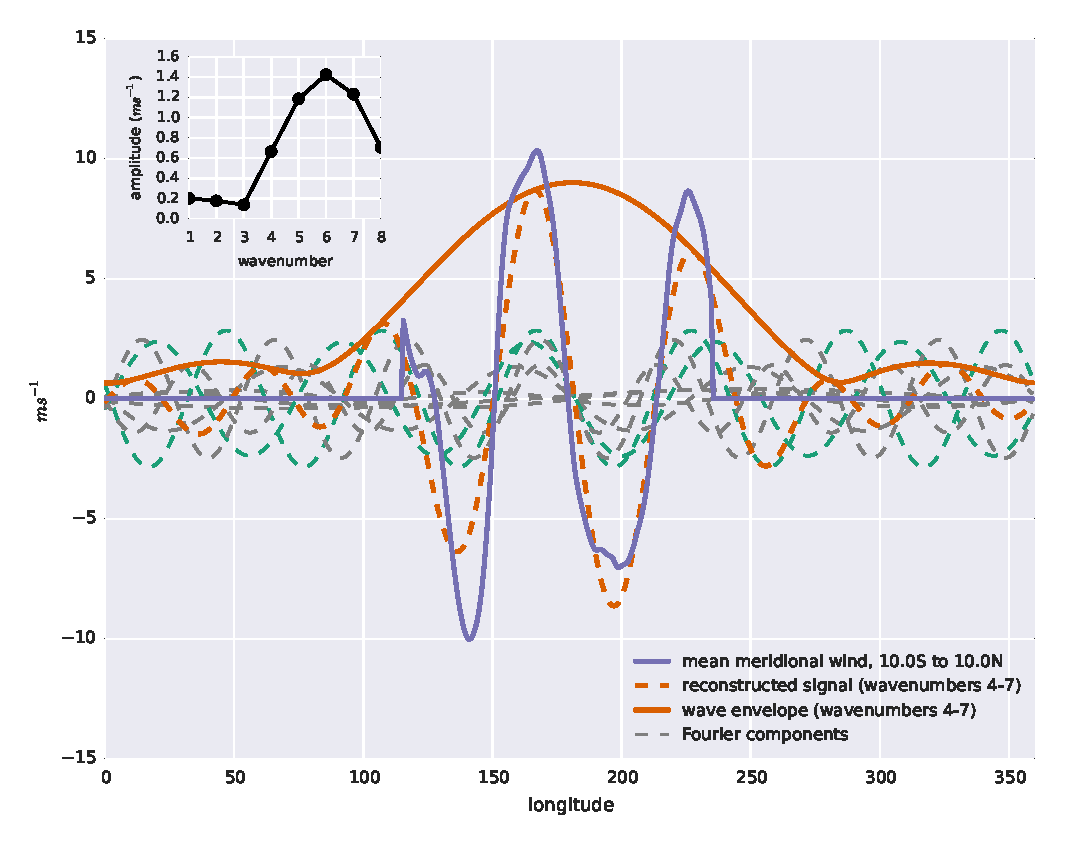
\includegraphics[width=0.84\columnwidth]{figures/psa/Figure4-2.eps}
\caption[Fourier analysis of the meridional average (10$^{\circ}$S to 10$^{\circ}$N) 500 hPa rotated meridional wind anomaly for a 30 day mean centred on 18 May 2006]{\label{fig:transform}
Fourier analysis of the meridional average (10$^{\circ}$S to 10$^{\circ}$N) 500 hPa rotated meridional wind anomaly for a 30 day mean centred on 18 May 2006 (purple curve). Values outside of the region of interest (115$^{\circ}$E to 235$^{\circ}$E) have been set to zero. The individual Fourier components for wavenumbers 1--8 (grey dashed, with wavenumbers five and six highlighted in green) and the reconstructed signal from an inverse Fourier transform with wavenumbers 4--7 retained (dashed orange) and its corresponding wave envelope (solid orange) are all shown. The inset shows the amplitude of each of the individual Fourier components.
}
\end{center}
\end{figure}

\subsubsection{Timescale considerations}

In applying the identification algorithm to the ERA-Interim dataset, this analysis focused on monthly timescale (i.e. 30 day running mean) data at 500 hPa. As with the zonal wave analysis, this atmospheric level was selected as it represents a mid-to-upper tropospheric level that is below the tropopause in all seasons and at all latitudes of interest. Given the equivalent barotropic nature of the PSA pattern (i.e. the wave amplitude increases with height but phase lines tend to be vertical) the results do not differ substantially for other levels of the troposphere. 

To explore the implications of this timescale selection, the Fourier transform used in the identification process was applied to the daily 500 hPa rotated meridional wind anomaly data for a number of different running mean windows (Figure \ref{fig:periodogram}). That analysis revealed wavenumber seven as the dominant frequency for daily timescale data in the PSA sector, with wavenumber six dominating the frequency spectrum for a 10--90 day running window. Given that the PSA pattern is itself characterised by wavenumber 5--6 variability in the PSA sector, this result suggests that (a) the PSA pattern is a dominant regional feature on weekly through to seasonal timescales, and (b) by extension the climatological results obtained from 30 day running mean data may also be relevant at those timescales.

\begin{figure}
\begin{center}
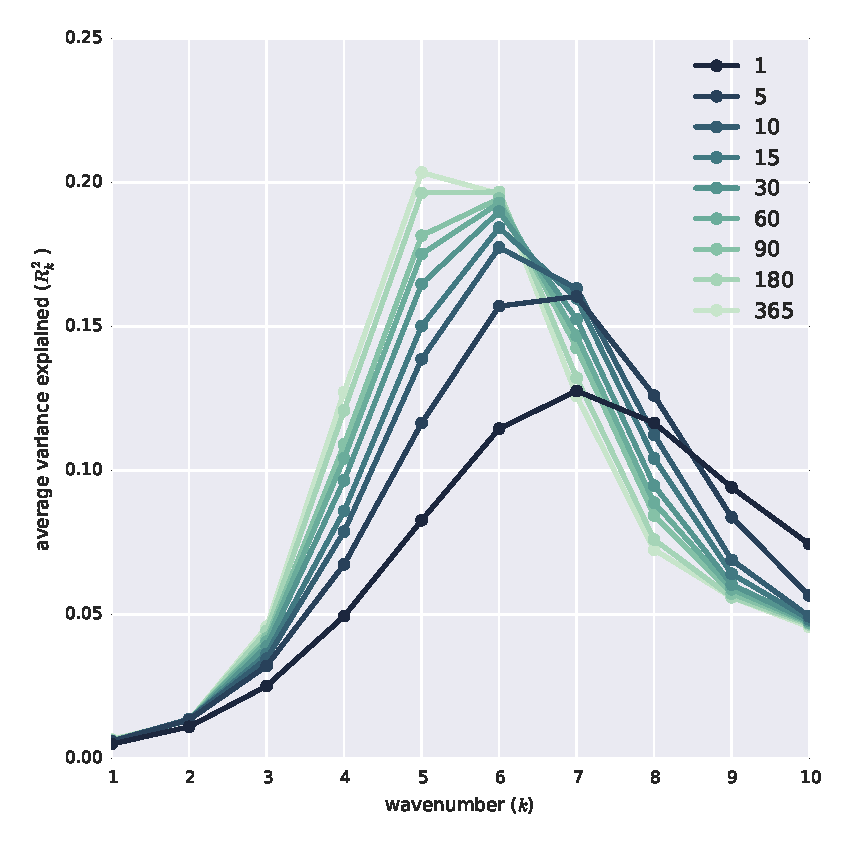
\includegraphics[width=0.7\columnwidth]{figures/psa/Figure4-3.eps}
\caption[Temporal average (1979--2014) periodograms for the meridional average (10$^{\circ}$S to 10$^{\circ}$N) 500 hPa rotated meridional wind anomaly]{\label{fig:periodogram}
Temporal average (1979--2014) periodograms for the meridional average (10$^{\circ}$S to 10$^{\circ}$N) 500 hPa rotated meridional wind anomaly (wind values outside of 115$^{\circ}$E to 235$^{\circ}$E were set to zero). Each curve represents a different running mean window that was applied to the daily timescale data prior to the analysis. The vertical axis units correspond to Equation \ref{eq:variance_explained}.%
}
\end{center}
\end{figure}


%=====================

\section{Results}

\subsection{General PSA-like variability}

Before attempting to isolate the PSA pattern using the phase information obtained from the identification algorithm, it is worth considering the characteristics of all PSA-like variability. In total, 55\% (7163 of 13120) of data times were identified as displaying PSA-like variability (i.e. wavenumber five and six were among the top three ranked frequencies), which is consistent with the fact that wavenumber six dominates the Fourier spectrum at the monthly timescale (Figure \ref{fig:periodogram}). Grouping consecutive identifications into discrete events revealed a mean event duration of 19.7 data times, with a distribution depicted in Figure \ref{fig:lifecycle}a. While interpretation of these duration data is complicated by the 30 day running mean applied to the original data (e.g. an event that lasted 10 data times could be said to span anywhere between 10 and 40 days) and the occurrence of short events immediately before or after a long event (i.e. they could conceivably be considered as a single event), it appears that PSA-like variability often persists for up to a few months at a time. Building on this baseline duration data, the life cycle of events lasting longer than 10 data times was investigated in more detail. As depicted in Figure \ref{fig:lifecycle}b, the amplitude of these events tended to peak mid-event, with some longer-lasting events peaking more than once during their lifetime (perhaps suggesting that some events simply merge into the next). The mean ($\pm$ standard deviation) linear phase trend across all events lasting longer than 10 data times was $0.12 \pm 0.38^{\circ}$E per data time, which indicates that while there was a tendency for events to propagate to the east, a substantial proportion moved very little or even towards the west during their lifetime. 

Important insights were also obtained by considering the phase distribution across all individual PSA-like data times (Figure \ref{fig:phase_distribution}). On an annual basis the distribution is clearly bimodal, with the two maxima of the kernel density estimate located at 12.75$^{\circ}$E and 45.0$^{\circ}$E. Since the phase was defined as the location of the first local maxima of the wavenumber six component of the Fourier transform, this approximate 30$^{\circ}$ phase separation indicates a pair of spatial patterns that are exactly out of phase (Figure \ref{fig:sf_composites}). Taken together these patterns clearly represent the single most dominant mode of variability in the PSA sector, and also closely resemble the PSA-1 mode identified by previous authors. On the basis of this finding, it appears that filtering the PSA-like data times according to the location of the two local maxima represents a simple and valid technique for isolating the PSA pattern from the larger population of PSA-like variability. 

The spatial patterns corresponding to the local minima of the phase distribution are also shown in Figure \ref{fig:sf_composites}, as a way to summarize the characteristics of the remaining PSA-like variability. The three anomaly centers associated with these composite mean circulation patterns have different amplitudes (the middle anomaly has a larger amplitude than the others), which indicates that it was often not a coordinated wave pattern that the identification algorithm was picking up (i.e. not the coordinated PSA-2 waveform discussed by previous authors, despite the similarity in wave phase). Looking at the individual data times corresponding to those minima (not shown), they appear to be a mixture of the hemispheric zonal wave three pattern \citep{Raphael2004,IrvingSimmonds2015}, a more meridionally oriented wave train extending from the tropical Pacific to the Amundsen Sea \citep[e.g.][]{Clem2015,Clem2015a} and isolated Amundsen Sea Low variability.


\begin{figure}
\begin{center}
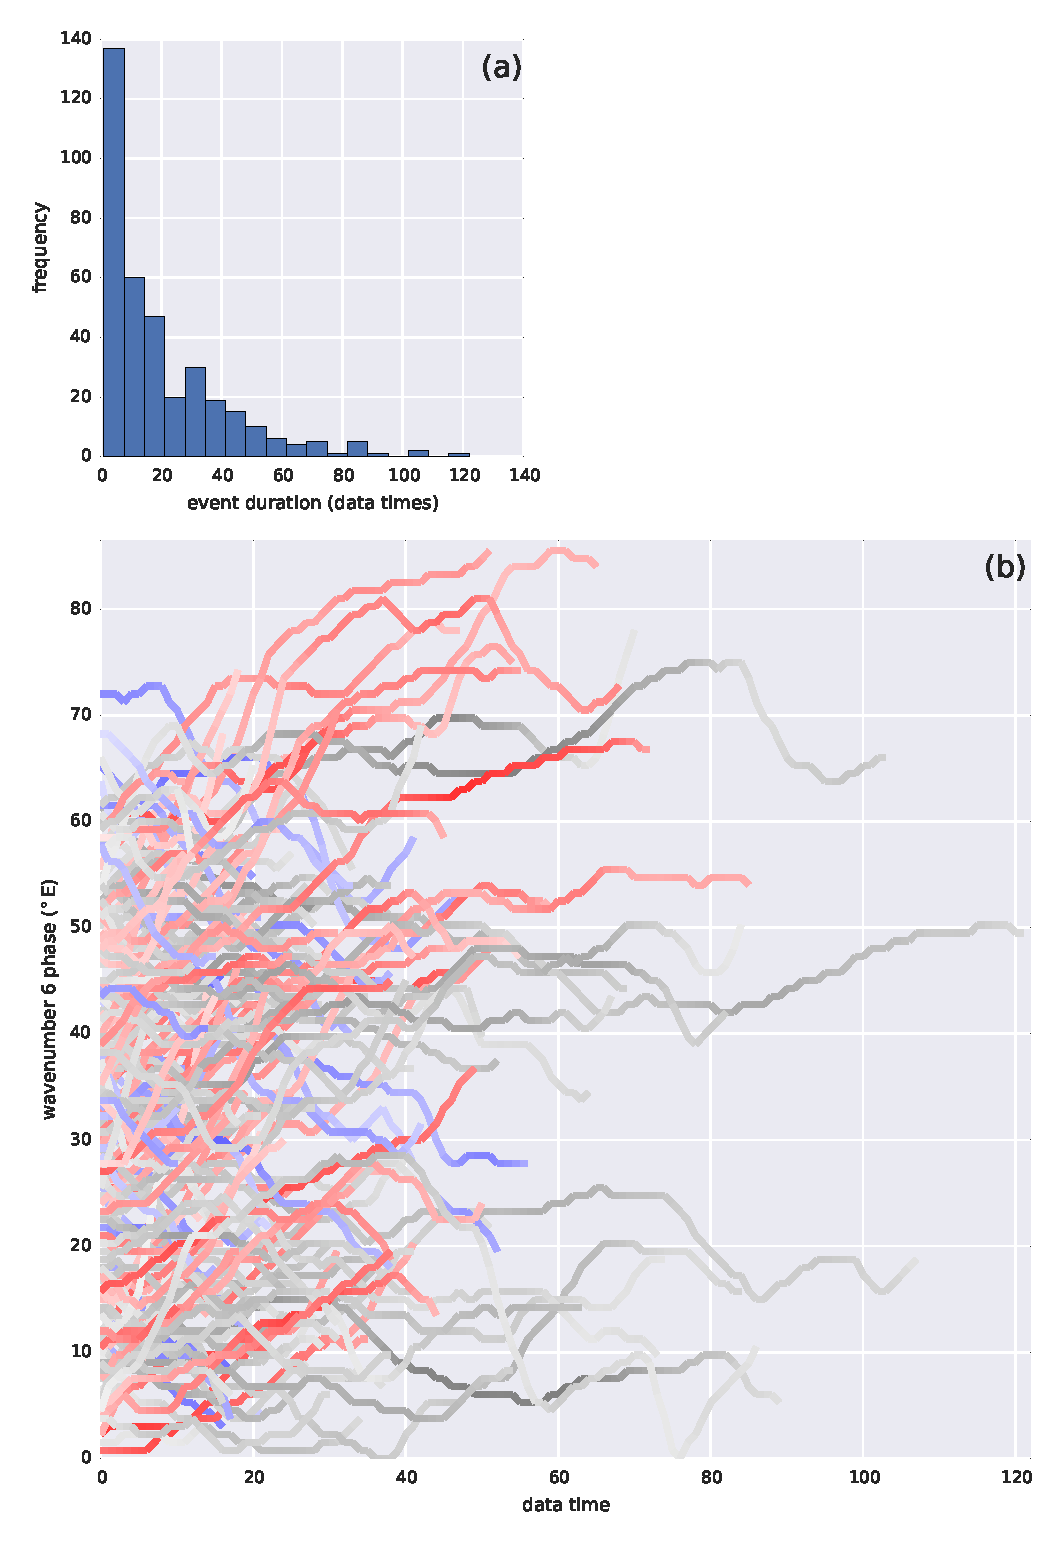
\includegraphics[width=0.8\columnwidth]{figures/psa/Figure4-4.eps}
\caption[Life cycle characteristics of PSA-like variability]{\label{fig:lifecycle}
Life cycle characteristics of PSA-like variability. The duration of all events is shown in panel (a), while the phase of events lasting more than 10 data times is shown in panel (b). Events that showed substantial eastward (defined as a linear phase gradient of greater than $0.25^{\circ}$E per data time) or westward (less than $-0.25^{\circ}$E per data time) propagation are coloured red and blue respectively, otherwise grey shading is used. The intensity of the shading represents the amplitude of the PSA-like variability. The maximum possible phase is $60^{\circ}$E, however for events that cross the cyclic 0/$60^{\circ}$E point the phase has been adjusted to ensure that a continuous line is maintained (e.g. a phase of $4^{\circ}$E would be converted to $64^{\circ}$E). %
}
\end{center}
\end{figure}

\begin{figure}
\begin{center}
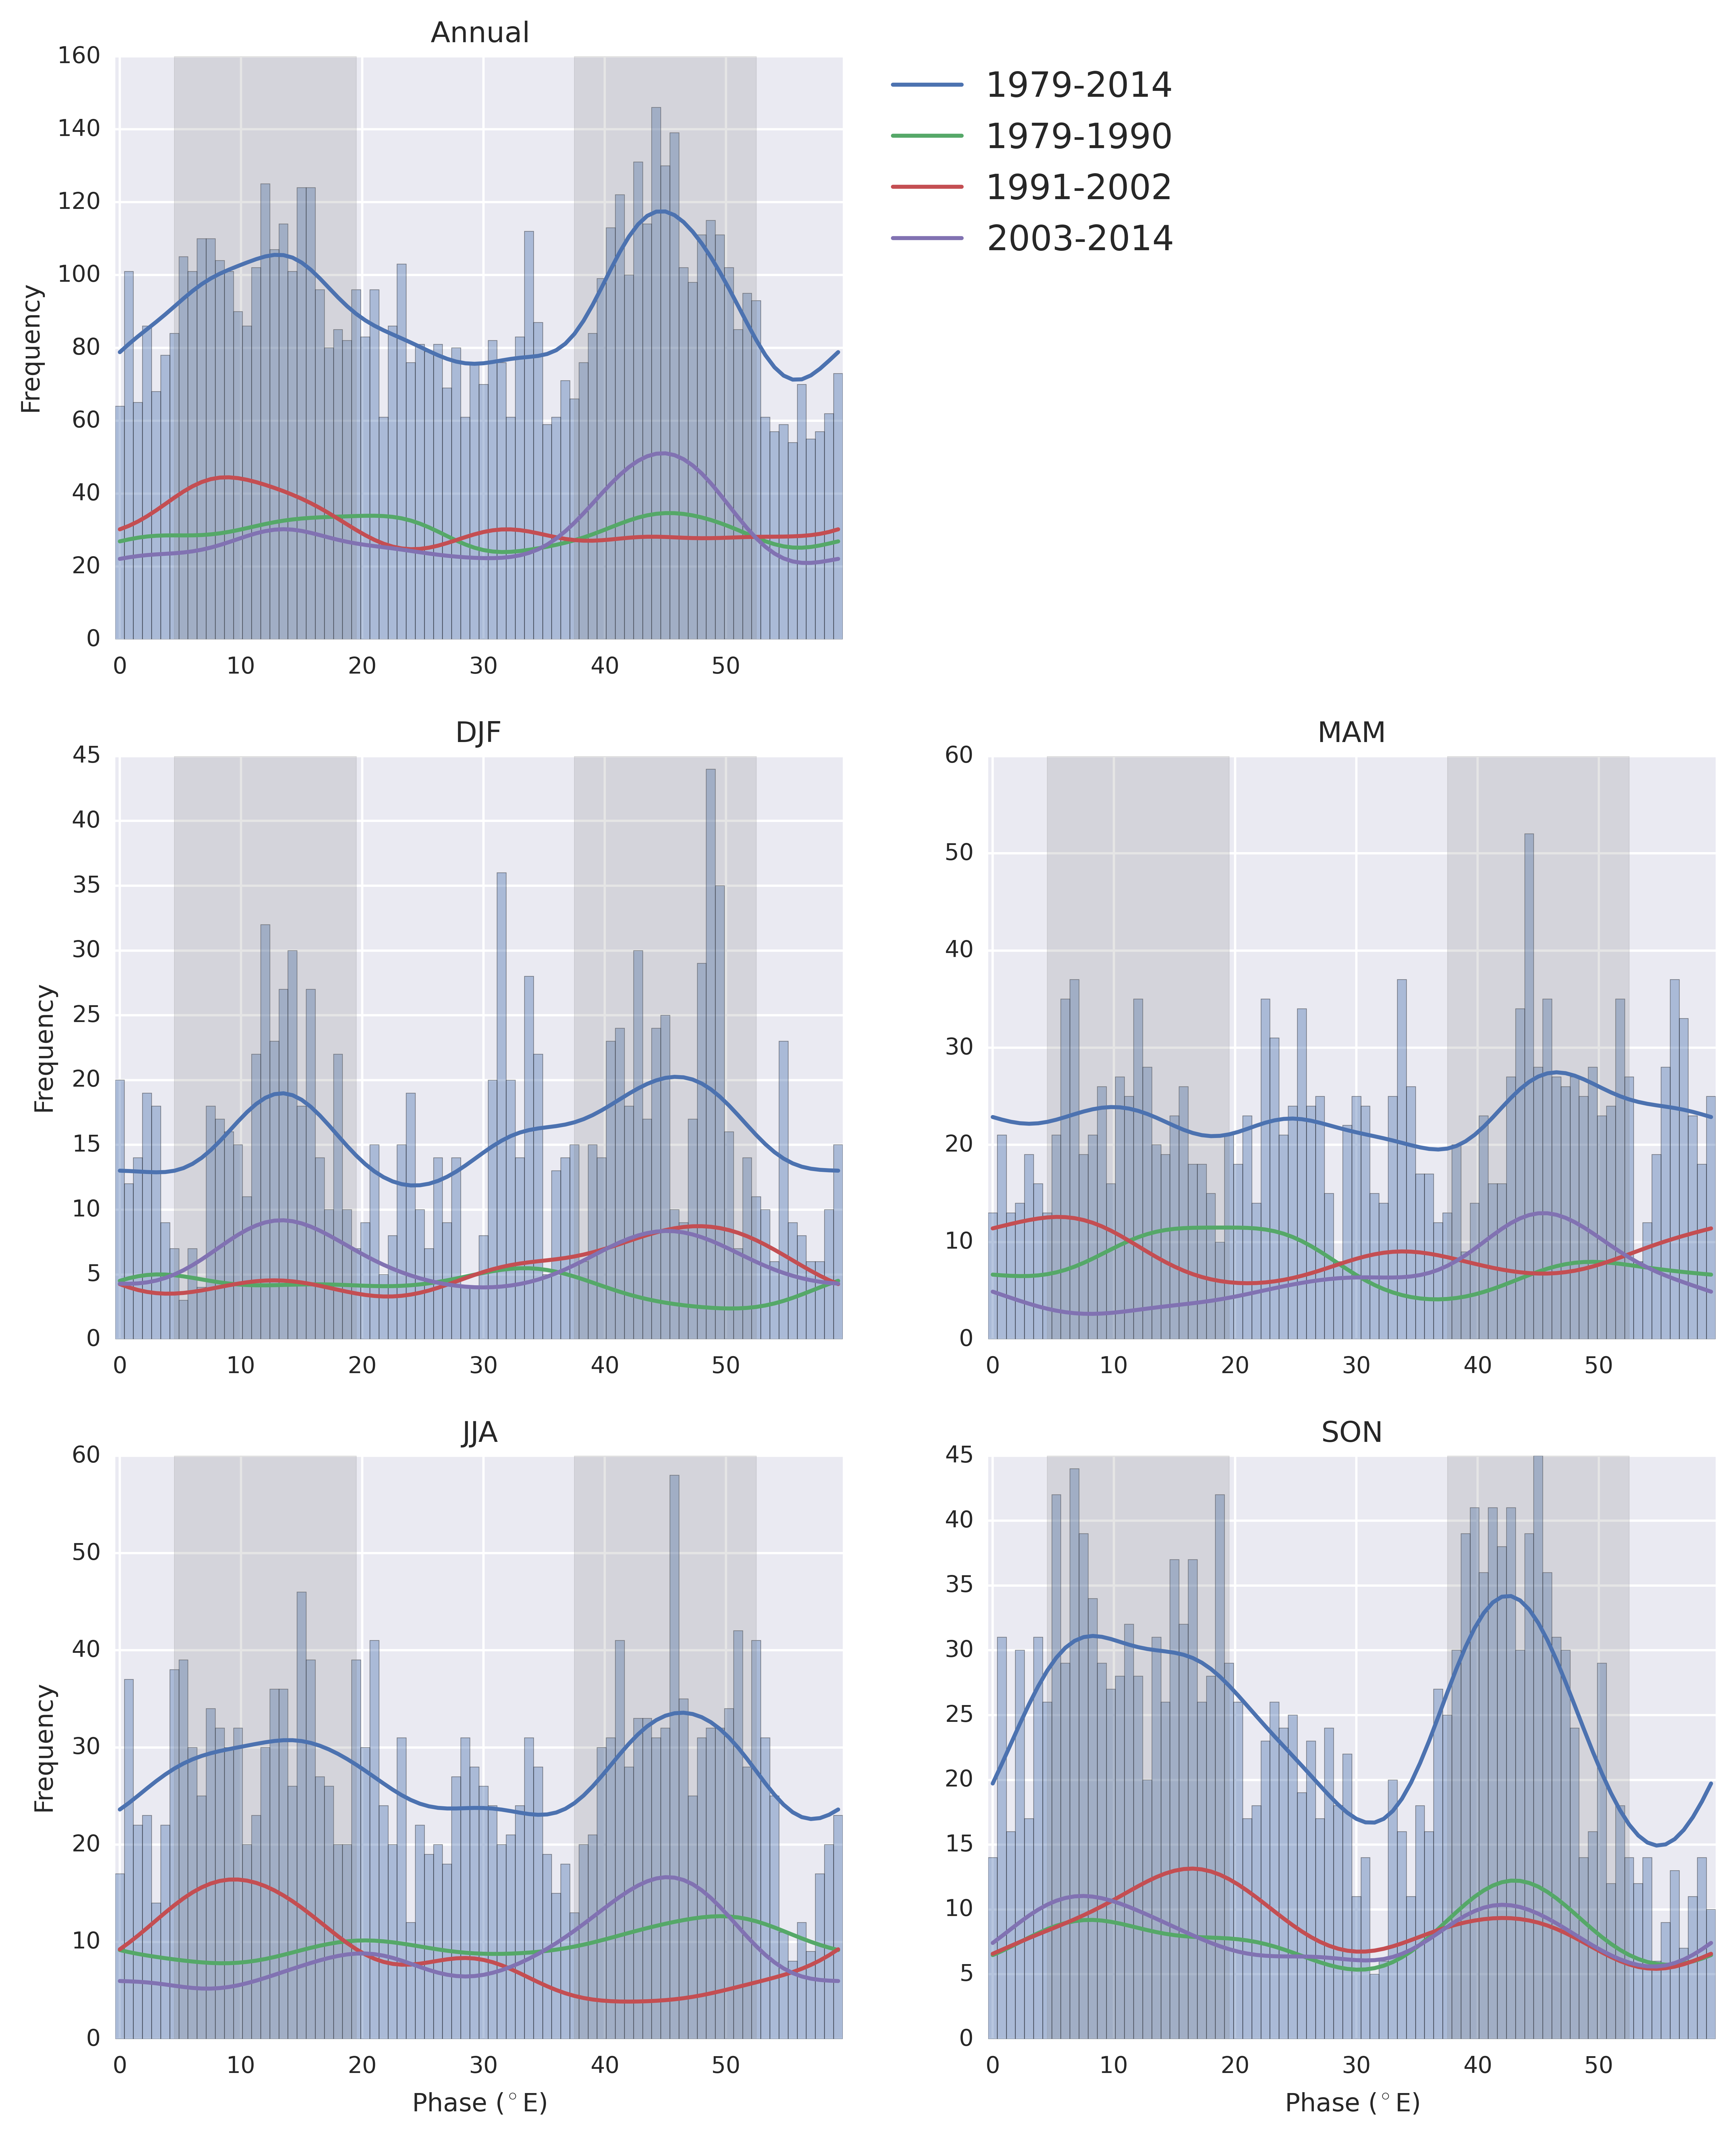
\includegraphics[width=0.98\columnwidth]{figures/psa/Figure4-5.png}
\caption[Phase distribution for all data times displaying PSA-like variability]{\label{fig:phase_distribution}
Phase distribution for all data times displaying PSA-like variability. The bars show the total count for each 0.75$^{\circ}$E interval over the period 1979--2014, while the lines represent kernel density estimates for a series of different time periods. Grey shading indicates the phase groupings taken to represent the positive (4.5 to 19.5$^{\circ}$E) and negative (37.5 to 52.5$^{\circ}$E) phase of the PSA pattern.%
}
\end{center}
\end{figure}

\begin{figure}
\begin{center}
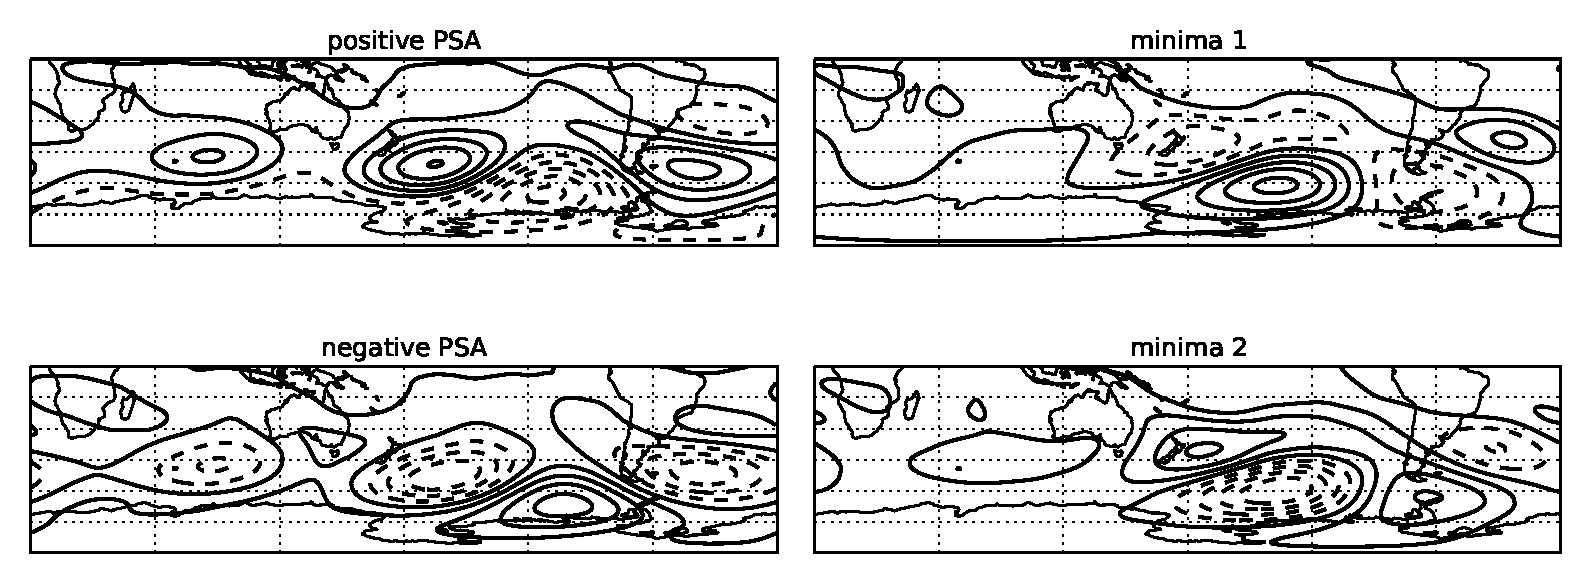
\includegraphics[width=1\columnwidth]{figures/psa/Figure4-6.eps}
\caption[Composite mean 500 hPa streamfunction anomaly for various phase groupings]{\label{fig:sf_composites}
Composite mean 500 hPa streamfunction anomaly for four different phase groupings: positive PSA pattern (4.5 to 19.5$^{\circ}$E), minima 1 (22.5 to 37.5$^{\circ}$E), negative PSA pattern (37.5 to 52.5$^{\circ}$E) and minima 2 (50.25 to 6.0$^{\circ}$E). Dashed contours indicate negative values and the contour interval is $1.5 \times 10^6 \: m^2 s^{-1}$.%
}
\end{center}
\end{figure}


\subsection{The PSA pattern}\label{s:psa_results}

In defining the PSA pattern according to the peaks of the PSA-like phase distribution, it was necessary to account for seasonal variations in the location of those peaks (Figure \ref{fig:phase_distribution}). A spread of 15$^{\circ}$ was considered sufficient to capture these variations, and hence the 15$^{\circ}$ interval about each local maxima containing the highest mean values (taken from the annual kernel density estimate) was determined. This approach was used to account of the fact that the phase histograms were not symmetrical about the local maxima and it yielded two intervals corresponding to the positive (4.5 to 19.5$^{\circ}$E) and negative (37.5 to 52.5$^{\circ}$E) phase of the PSA pattern. Both intervals represented approximately 15\% of all data times (14.8\% for the positive phase versus 15.8\% for the negative), which suggests that the two phases have a similar frequency of occurrence. With this definition in place, it was possible to investigate variability and trends in the PSA pattern as well as its influence on surface temperature, precipitation and sea ice. 

\subsubsection{Trends and variability}

During autumn and winter in particular, the middle years of the study period (1991--2002) were characterised by a predominance of positive PSA pattern activity, while negative phase activity was more common in recent years (Figure \ref{fig:phase_distribution}). This variability is reflected in the linear trends observed over 1979--2014, with negative phase activity showing a statistically significant increasing trend (at the $p < 0.05$ level) on an annual basis and smaller non-significant increasing trends for summer, autumn and winter (Figure \ref{fig:psa-neg_seasonality}). Positive phase activity showed a non-significant decreasing trend on an annual basis and also during autumn and winter, with an increasing trend observed for summer (Figure \ref{fig:psa-pos_seasonality}). Both phases of the PSA pattern were most active during winter and spring (Figure \ref{fig:psa-neg_seasonality} and \ref{fig:psa-pos_seasonality}). 

\begin{figure}
\begin{center}
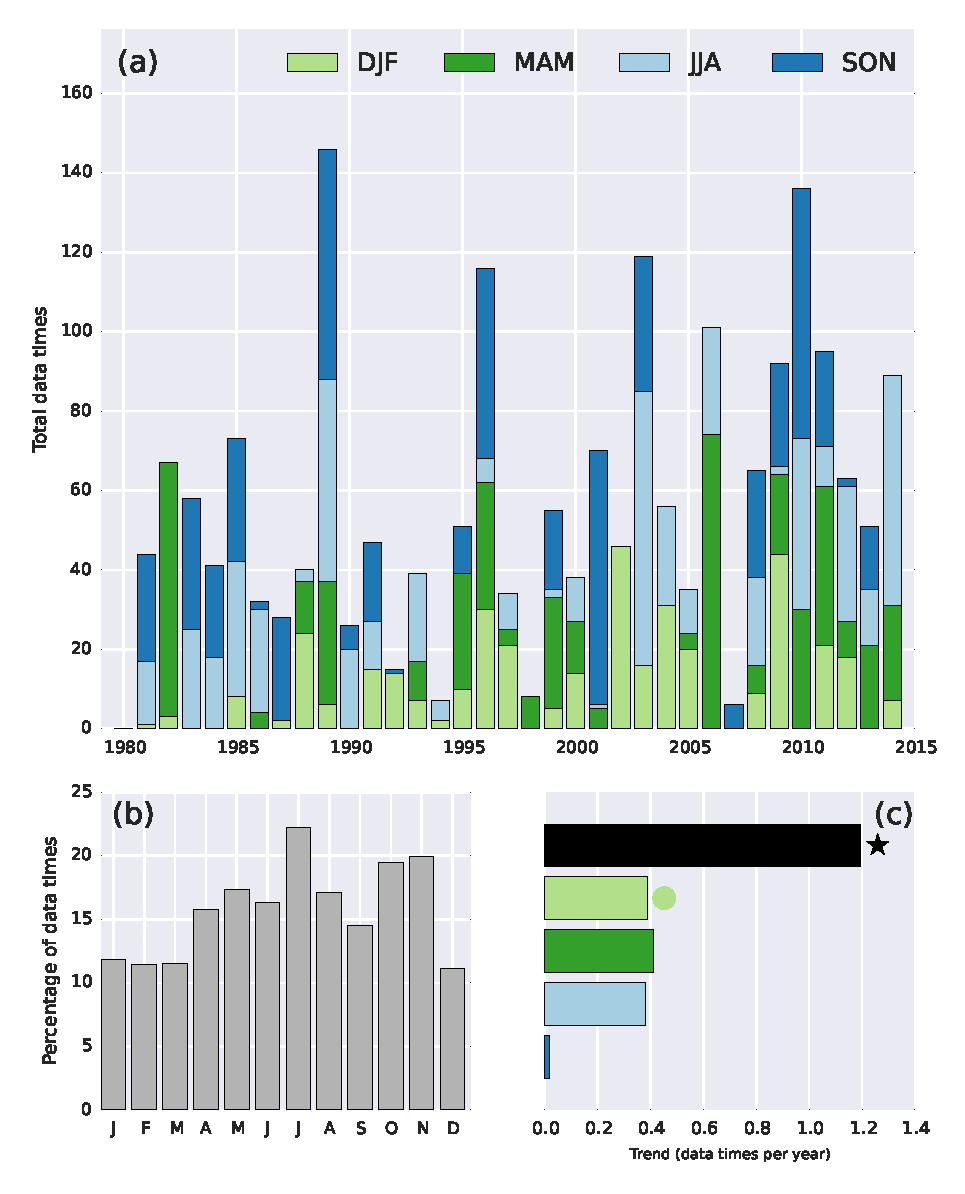
\includegraphics[width=0.9\columnwidth]{figures/psa/Figure4-7.eps}
\caption[Variability and trends in the negative phase of the PSA pattern]{\label{fig:psa-neg_seasonality}
Variability and trends in the negative phase of the PSA pattern. The total PSA-negative data times for each individual season are shown in panel (a), corresponding seasonal linear trends in panel (c) (black represents the annual trend) and monthly totals for the entire study period (1979--2014) in panel (b). To account for the fact that not all months have an equal number of days, the counts for each month in panel (b) are presented as a percentage of the total number of days for that month. Years in panel (a) are defined from December to November (e.g. the `year' 1980 spans December 1979 to November 1980) and trends that are statistically significant at the $p < 0.10$ and $p < 0.05$ level are indicated with a circle and star respectively.%
}
\end{center}
\end{figure}

\begin{figure}
\begin{center}
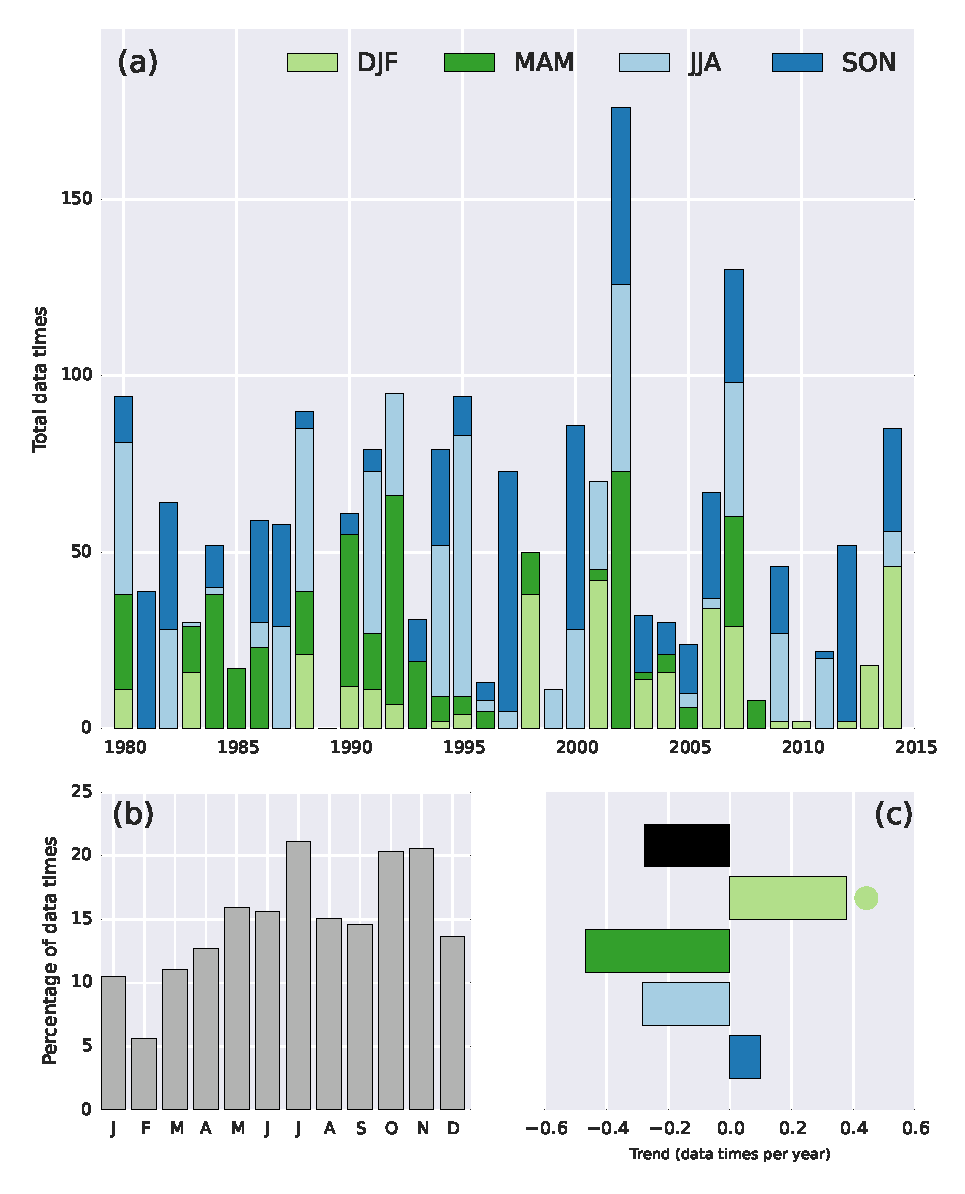
\includegraphics[width=0.9\columnwidth]{figures/psa/Figure4-8.eps}
\caption[Variability and trends in the positive phase of the PSA pattern]{\label{fig:psa-pos_seasonality}
As per Figure \ref{fig:psa-neg_seasonality} but for the positive phase of the PSA pattern.%
}
\end{center}
\end{figure}


In attempting to explain annual and decadal variability in the PSA pattern, previous authors have suggested that coupling between the SAM and ENSO is important \citep[e.g.][]{Fogt2006}. While some degree of coupling is evident in Figure \ref{fig:sam_v_enso} (i.e. the positive phase of the PSA pattern was most common when positive ENSO events and negative SAM events coincided), it is clear that the SAM has a much stronger association with PSA pattern activity than ENSO. Recent positive trends in the SAM during summer, autumn and to a lesser extent winter \citep[the latter being smaller and not statistically significant; e.g.][]{Simmonds2015} are also broadly consistent with the negative trends observed in the PSA pattern during those seasons.  

\begin{figure}
\begin{center}
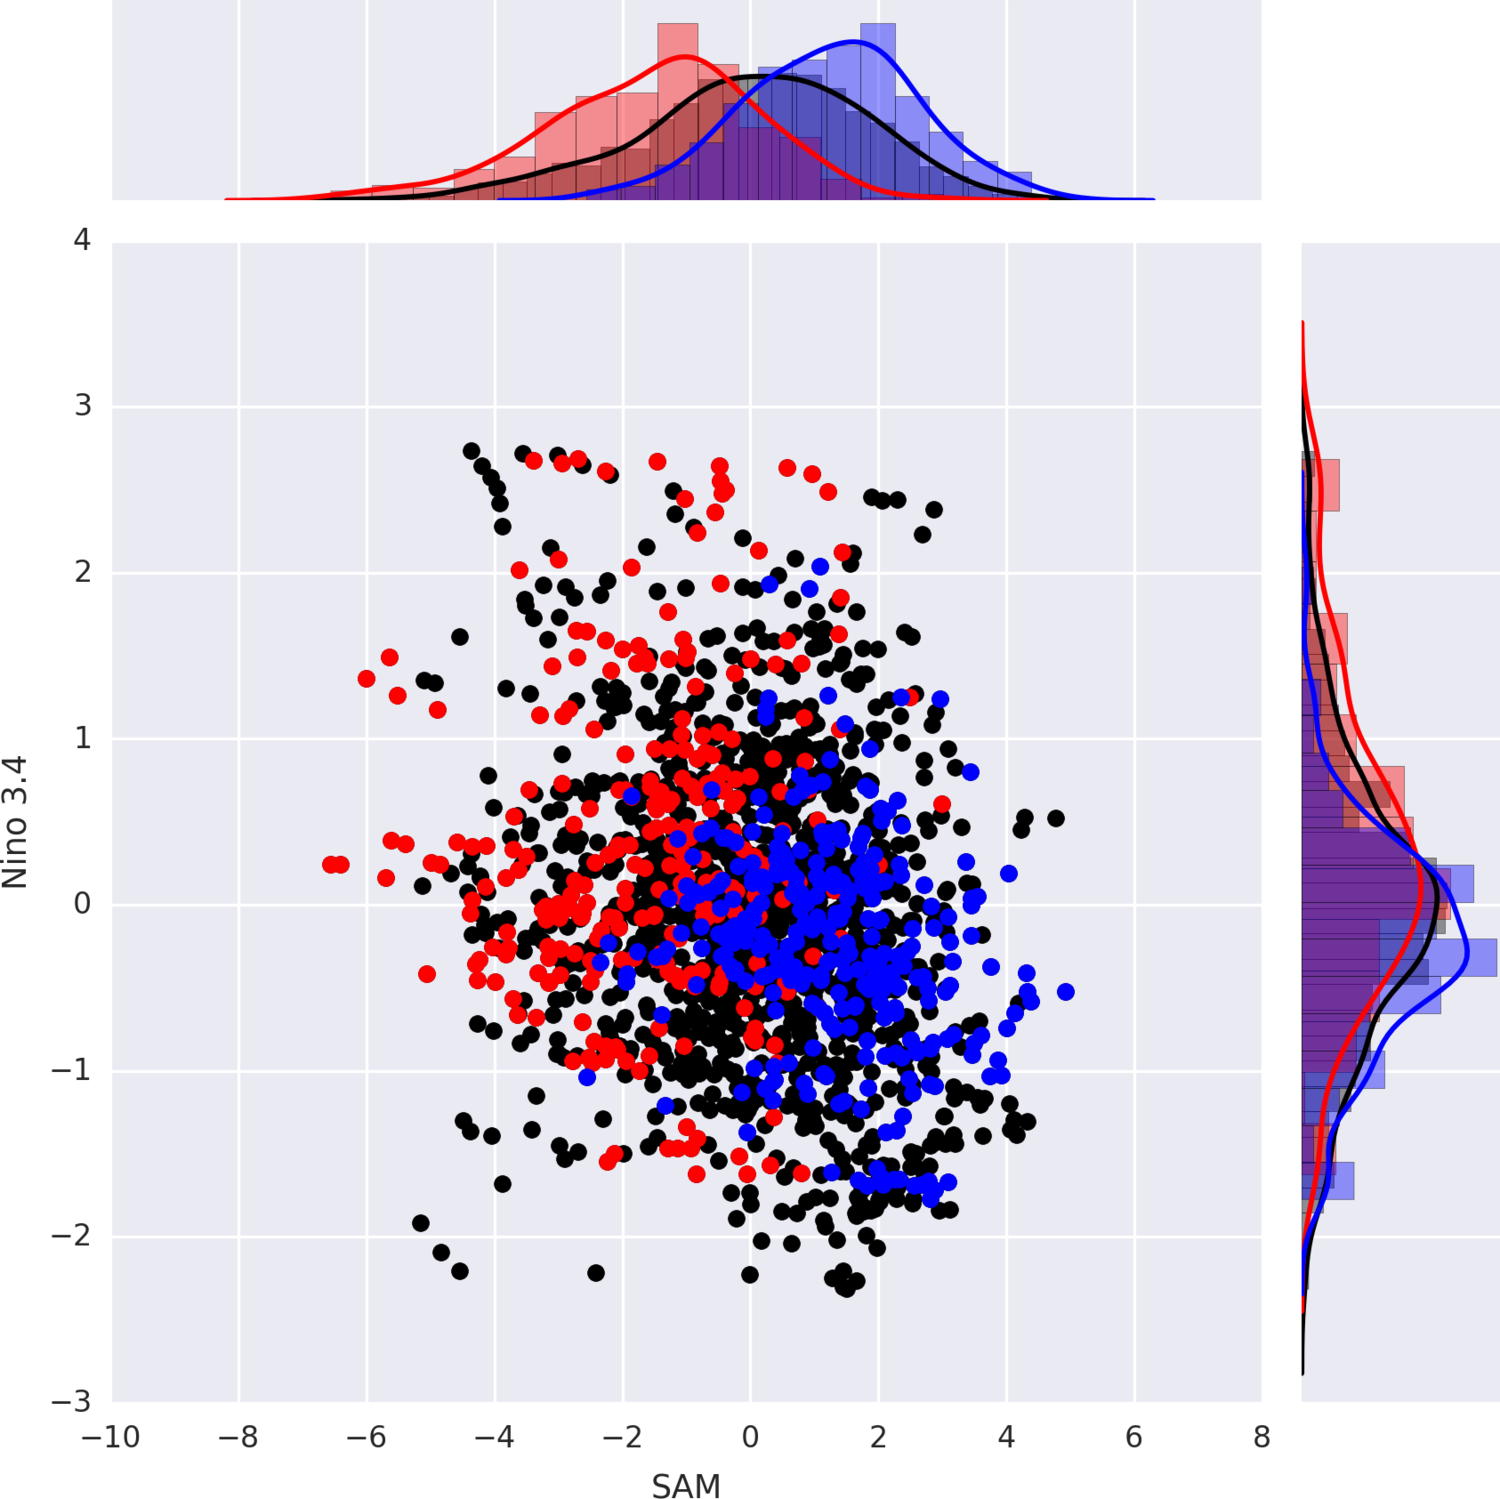
\includegraphics[width=0.8\columnwidth]{figures/psa/Figure4-9.png}
\caption[SAM versus Ni\~{n}o 3.4 for various temporal subsets]{\label{fig:sam_v_enso}
SAM versus Ni\~{n}o 3.4 for all data times (shown in black) over the period 1979--2014. Dots corresponding to PSA-positive and PSA-negative data times were re-coloured red and blue respectively and were arranged in the following order from front to back: blue, red, black (i.e. a blue dot might have red and/or black dots hidden underneath). For clarity, only every seventh data time was plotted. Corresponding histograms and kernel density estimates for the SAM (top panel) and Ni\~{n}o 3.4 (right panel) are shown and have been scaled according to density as opposed to frequency (hence the amplitudes are comparable).%
}
\end{center}
\end{figure}

\subsubsection{Influence on surface variables} 

In order to assess the influence of the PSA pattern on regional climate variability, the composite mean surface air temperature anomaly, precipitation anomaly and sea ice concentration anomaly was calculated for both the positive and negative phase (Figure \ref{fig:surface_composites}). On the western flank of the central composite mean streamfunction anomaly associated with positive phase activity, anomalously warm conditions were evident over the Ross Sea, Amundsen Sea and interior of West Antarctica, particularly during autumn and winter. The northerly flow responsible for these warm conditions also induced large precipitation increases along the West Antarctic coastline and reduced sea ice in the Amundsen Sea. On the eastern flank, anomalously cool conditions were evident over the Antarctic Peninsula, Patagonia and the Weddell Sea during all seasons (winter and spring especially), with the latter also experiencing large increases in sea ice. Anomalously dry conditions were also seen over the Antarctic Peninsula in association with the weaker westerly flow. 

The anomalies associated with the negative phase of the PSA pattern were essentially the reverse of the positive phase (Figure \ref{fig:surface_composites}). It is also noteworthy that while the hemispheric composite mean streamfunction anomaly associated with the PSA pattern gives the impression of a hemispheric ZW3 pattern, the phase of that pattern and the unremarkable anomalies either side of the Indian Ocean anomaly are inconsistent with the characteristics of the dominant ZW3 mode (Chapter \ref{c:zw_climatology}).

\begin{figure}
\begin{center}
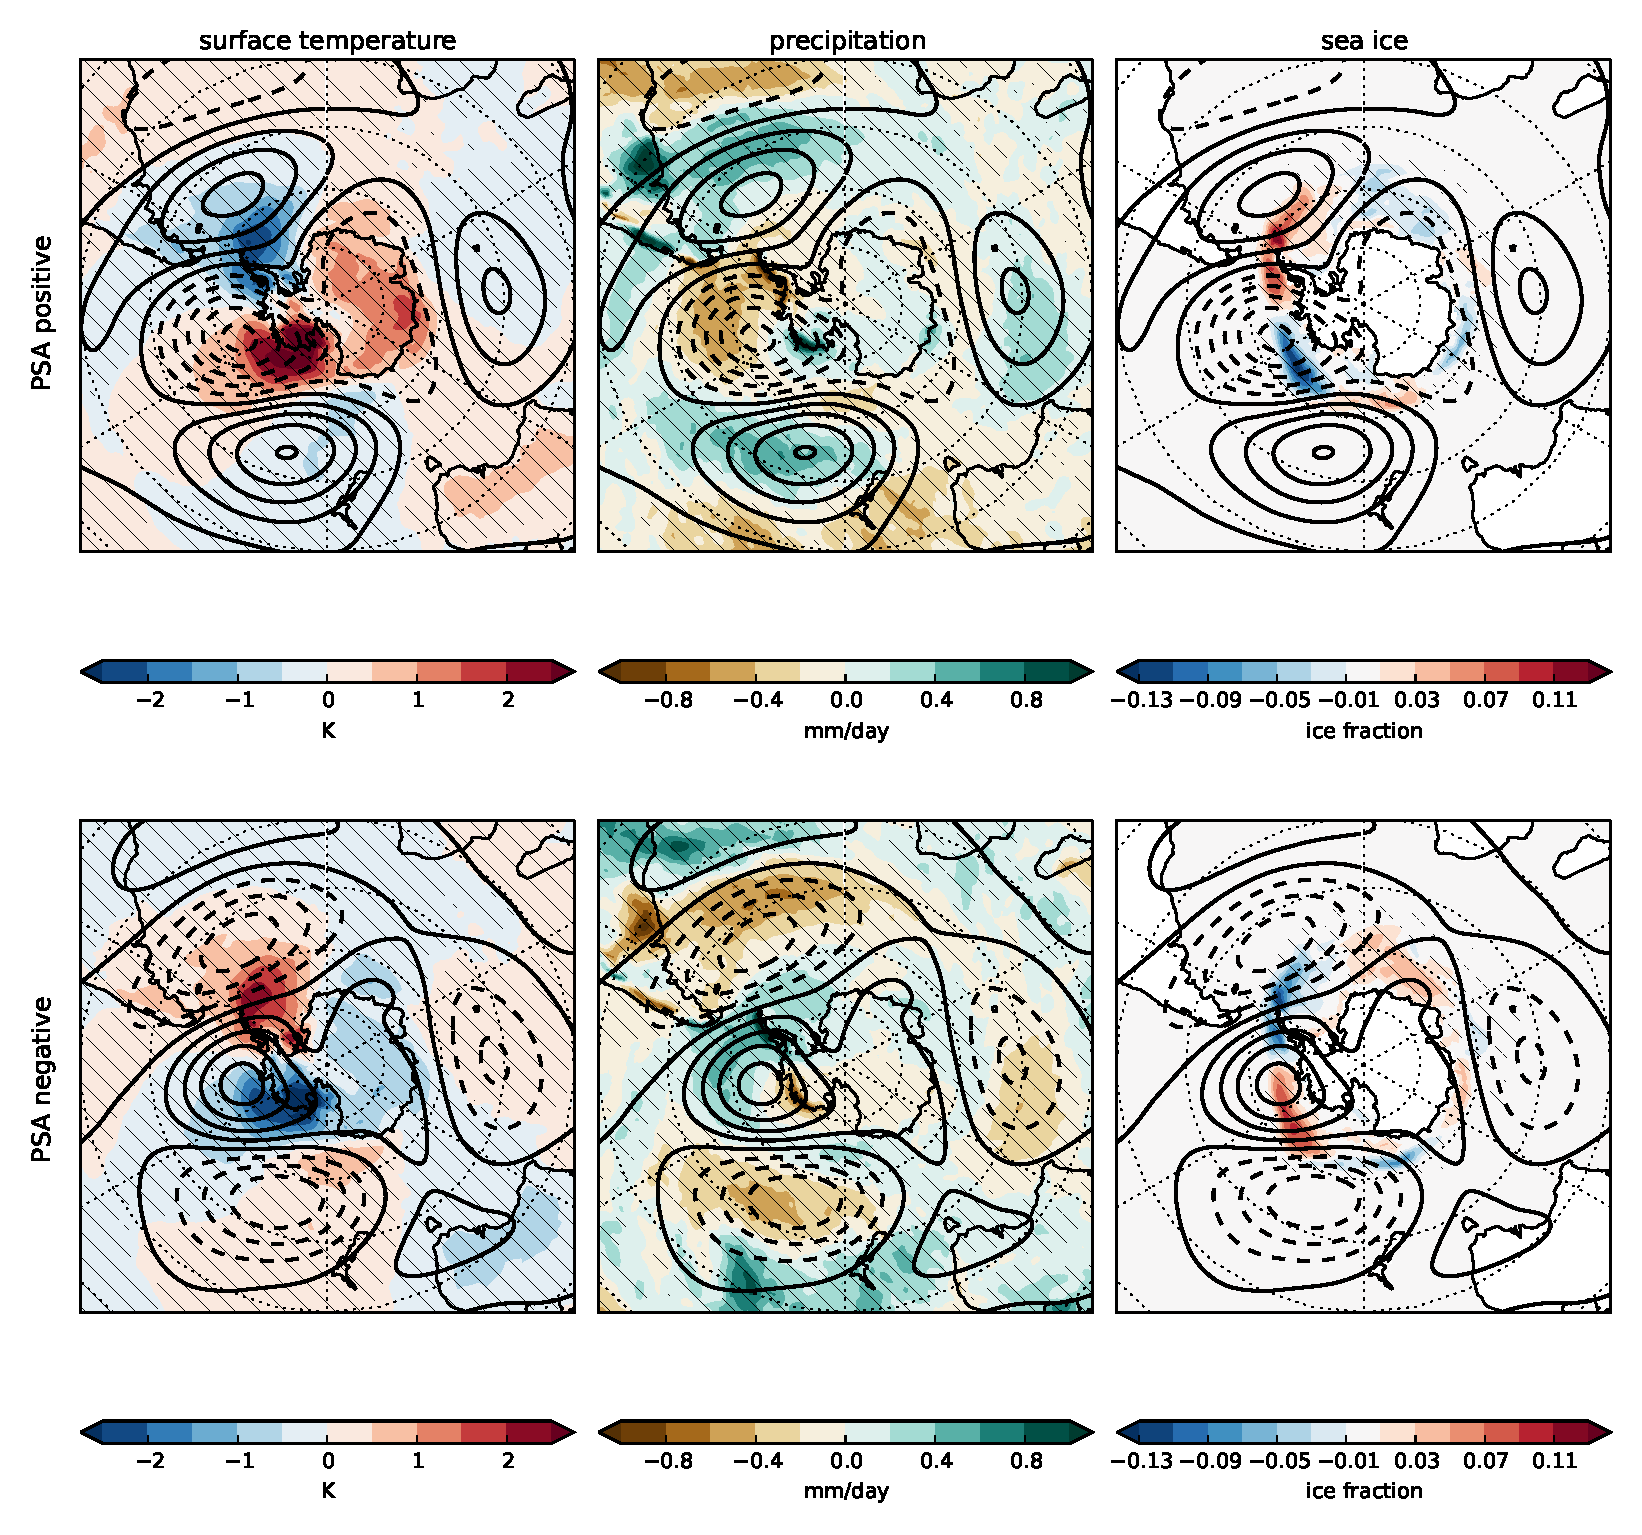
\includegraphics[width=1\columnwidth]{figures/psa/Figure4-10.eps}
\caption[Composite mean surface air temperature anomaly, precipitation anomaly and sea ice fraction anomaly for all data times corresponding to the positive or negative phase of the PSA pattern]{\label{fig:surface_composites}
Composite mean surface air temperature anomaly, precipitation anomaly and sea ice fraction anomaly for all data times corresponding to the positive (phase grouping 4.5 to 19.5$^{\circ}$E; top row) or negative (37.5 to 52.5$^{\circ}$E; bottom row) phase of the PSA pattern. Black contours show the composite mean 500 hPa streamfunction anomaly (dashed contours indicate negative values and the contour interval is $1.5 \times 10^6 \: m^2 s^{-1}$), while the hatching shows regions where the difference between the composite mean and climatological mean is significant at the $p < 0.01$ level.%
}
\end{center}
\end{figure}


%=====================

\section{Discussion}

A novel methodology has been presented for objectively identifying the PSA pattern. By rotating the global coordinate system such that the equator (a great circle path) traces the approximate path of the PSA pattern, the method was able to utilise Fourier analysis to quantify the phase and amplitude of wave-like variability in the PSA sector. In reconciling the results of this Fourier analysis with existing EOF-based definitions of the PSA pattern, a strong resemblance was found between the existing PSA-1 mode and the spatial pattern corresponding to the bimodal phase peaks of wavenumber 5--6 dominant variability in the PSA sector. The lack of a higher-order, multi-modal phase distribution questions the physical reality of the existing PSA-2 mode, and may explain the difficulty that researchers have had in identifying a tropical driver for that mode.     

These bimodal phase peaks were used as a means to define the positive and negative phase of the PSA pattern. The climatology arising from this definition revealed that the PSA pattern is most active during winter and spring, often persisting for months at a time. It propagates to the east on average, but a substantial number of events remain relatively stationary or even propagate to the west. The pattern was also shown to have a strong influence on regional temperature, precipitation and sea ice variability. With respect to the former, the results confirm existing relationships established between pattern and station temperatures over the Antarctic Peninsula \citep[e.g.][]{Schneider2012,Yu2012}, extending the regional picture to highlight equally strong temperature anomalies (of opposite sign) over West Antarctica. Large precipitation anomalies were also identified along the coast of West Antarctica and the Antarctic Peninsula, as well as over South America. These South American anomalies show a more complex spatial pattern than previous analyses (perhaps due to the higher resolution data), but are otherwise broadly consistent with the results of \citet{Mo2001}, who found the positive phase of the PSA pattern to be associated with anomalously wet conditions over southern South America and anomalously dry conditions further north. Previous studies also indicate that the PSA pattern plays an important role in sea ice variability in the Amundsen and Bellingshausen Seas \citep{Raphael2014}. The results presented here suggest that this role is not uniform across that region, with composites of the positive phase of the PSA pattern simultaneously displaying positive sea ice anomalies in the Bellingshausen Sea and negative in the Amundsen Sea.  

With respect to trends in the PSA pattern over the period 1979--2014, a trend towards the negative phase was identified on an annual basis and also during summer, autumn and winter. This autumn trend (and the high latitude temperature and sea ice anomalies associated with the negative phase of the PSA pattern) is consistent with the work of \citet{Ding2013}, who found that autumn warming over the Antarctic Peninsula and associated sea ice declines over the Bellingshausen Sea are associated with an atmospheric circulation resembling the negative phase of the PSA pattern. While this explanation makes sense on the eastern flank of the central circulation anomaly associated with that pattern, the negative phase of the PSA pattern is also associated with strong cooling over West Antarctica. Autumn temperature declines have not been observed in that region, and thus results presented here suggest that the PSA-related cooling must have been offset by other factors. 

In contrast to the autumn warming over the Antarctic Peninsula, winter warming over West Antarctica has been associated with an atmospheric circulation resembling the positive phase of the PSA pattern \citep{Ding2011}. The climatology presented here revealed a (albeit non-significant) trend towards the negative phase of the PSA pattern during winter, which raises the question: how is it that winter temperature trends over West Antarctica are associated with an atmospheric circulation resembling the positive phase of the PSA pattern, but a climatology of PSA pattern activity reveals a trend that directly opposes that finding? One possible answer to this question comes from \citet{Li2015a}. They analysed Rossby wave trains associated with observed SST trends in the tropical Atlantic, tropical Indian, west Pacific and east Pacific regions and found that all four have a center of action over the Amundsen Sea. While none of these individual wave trains resembled the PSA pattern, a linear combination of the four of them did (with the tropical Atlantic and west Pacific identified as most influential). In other words, the integrated influence of tropical SST trends on the atmospheric circulation resembles the positive phase of the PSA pattern, but the waves underpinning that teleconnection do not. This result is consistent with an earlier study that identified the tropical Atlantic as a driver of recent winter trends in West Antarctica \citep{Li2014}. Another possible answer comes from \citet{Fogt2015}, who suggest that radiative forcing has played a role in Amundsen Sea Low trends that are consistent with winter warming in West Antarctica. The absence of any springtime trend in the PSA pattern suggests that it has also not played a role in high latitude warming during that season. Similar to winter, the Atlantic has been linked to warming in West Antarctica during spring \citep{Simpkins2014}, while others point to a more meridionally oriented wave train associated with the Pacific Decadal Oscillation \citep[PDO;][]{Clem2015,Clem2015a}. 

This idea that radiatively forced Amundsen Sea Low variability and/or wave trains associated with the Atlantic or PDO might be responsible for a teleconnection resembling the PSA pattern (i.e. as opposed to changes in actual PSA pattern activity) goes to the heart of the reversibility argument made in Section \ref{s:psa_overview}. For a proposed teleconnection to be robust, it must be evident when looking through the lens of both the variable and mechanism of interest. However, even if these alternative explanations do reconcile the discrepancy between the climatology presented here and winter warming over West Antarctica, the associated circulation anomaly would bring cooler conditions and wind-driven increases in sea ice along the western Antarctic Peninsula, contrary to the observed warming and sea ice declines \citep{Clem2015}. One possible explanation is that the negative autumn sea ice anomalies persist into winter \citep{Ding2013}, however it is clear that there is still work to be done to fully understand recent winter temperature and sea ice changes in the region.

One topic not addressed here is variability in the east/west location of the PSA pattern. In response to the emergence of central Pacific ENSO events in recent years \citep[e.g.][]{Ashok2007}, some authors have suggested that the PSA pattern moves east/west depending on the precise location of the associated tropical SST anomalies \citep[e.g.][]{Sun2013,Wilson2014,Ciasto2015}. Others suggest that the pattern is relatively stationary \citep[e.g.][]{Liu2007,Ding2012}, however either way the broad region (10$^{\circ}$N to 10$^{\circ}$S in the rotated coordinate system) used by the identification algorithm developed here renders it insensitive to subtle east/west movements. Given that the PSA pattern did not show a strong association with the Ni\~{n}o 3.4 index (an index that is sensitive to both central and eastern Pacific ENSO events), it would be fair to say that even if the location of tropical SSTs does cause the pattern to move slightly, this would represent only a small fraction of all PSA pattern activity. 

This weak association with ENSO challenges our fundamental understanding of the PSA pattern. The most commonly held view to date is that the pattern is primarily a response to ENSO forcing \citep[e.g.][]{Mo2001}, whereby anomalous ENSO-related SST anomalies modify tropical convection, leading to atmospheric vorticity gradients conducive to Rossby wave generation \citep{Sardeshmukh1988}. A more comprehensive analysis of the relationship between the pattern and tropical convection would be required to confirm this (e.g. lagged correlations with SSTs and other indicators of tropical convection like the outgoing longwave radiation), but the result presented here suggest that the PSA pattern might actually be better conceptualised as a preferred regional atmospheric response to various internal and external forcings (i.e. with ENSO being just one of many players). Tropical convection is almost certainly an important factor, but its role is likely more complicated than can be captured by a broad-scale ENSO index like the Ni\~{n}o 3.4. This complex relationship between tropical SSTs, convection and the PSA pattern has been the focus of a small number of studies \citep[e.g.][]{Harangozo2004,LachlanCope2006} and is a topic that warrants much more attention. The relationship between the PSA pattern and ENSO has also traditionally been thought to be moderated by the state of the `atmospheric bridge' \citep{Liu2007}. In particular, the pattern is thought to be most active when ENSO and the SAM are in phase \citep{Fogt2006}. Rather than casting the SAM in a facilitating/bridging role, the strong association identified here is more consistent with the idea that the PSA pattern is an integral part of the zonally asymmetric structure of the SAM \citep[e.g.][]{Ding2012,Fogt2012}. 
